\setcounter{chapter}{5}
\setcounter{section}{0}
\setcounter{figure}{0}   
\chapter*{Discussion}         % ne pas numéroter
\phantomsection\addcontentsline{toc}{chapter}{Discussion} % dans TdM

\section{Apport des travaux et retour critique}

\subsection{GWENA}

Les travaux de ce doctorat ont débutés dans un contexte où l'analyse par réseaux de co-expression, bien qu'existante depuis plus de 15 ans, n'était pas aussi démocratisé qu'elle l'aurait pu au vu des bénéfices qu'elle apporte (Figure \ref{fig:count_by_year_coexpr_diff_expr}). Pour contribuer à sa démocratisation et plus particulièrement à la celle de la co-expression différentielle, le progiciel R GWENA a été développé avec comme objectif d'être facilement utilisable et de contenir de nombreux avertissements sur un mésusage. Son dépôt sur le répertoire Bioconductor complétait cette volonté car celui-ci constitue une référence en bio-informatique et favorise une meilleure visibilité. Il assure également une qualité plus haute qu'un package déposé sur l'autre répertoire populaire, le CRAN, grâce à un contrôle qualité du code bien plus strict et une obligation de maintenance et réponse aux demandes des utilisateurs.

\begin{figure}[h]
    \centering
    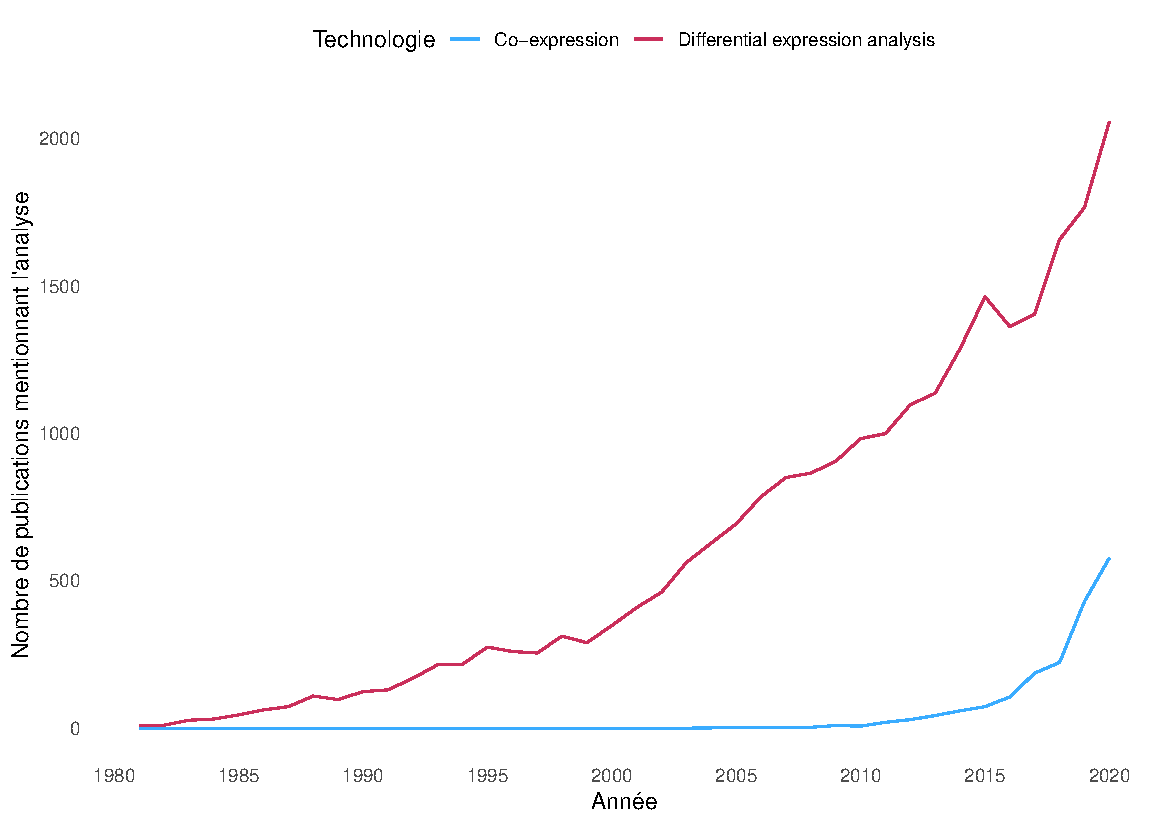
\includegraphics[width=1\textwidth]{img/intro/discu/count_by_year_coexpr_diff_expr.pdf}
    \caption[Évolution de l'utilisation de l'analyse d'expression différentielle et l'analyse par réseaux de co-expression de gènes en se basant sur le nombre de publications les mentionnant]{Évolution de l'utilisation de l'analyse d'expression différentielle et l'analyse par réseaux de co-expression de gènes en se basant sur le nombre de publications les mentionnant. Les résultats proviennent du site PubMed (\url{https://pubmed.ncbi.nlm.nih.gov}) avec les requêtes suivantes : \textbf{Expression différentielle} = "differential expression" analysis, \textbf{Co-expression} = "gene co-expression network"}
    \label{fig:count_by_year_coexpr_diff_expr}
\end{figure}

Cependant d'autres outils existaient déjà pour des usages similaires bien que moins complets. Une étude des besoins d'analyse via une revue de nombreux article utilisant ces différents outils a amené à plusieurs choix et ajouts dans GWENA. L'ajout majeur réside dans l'implémentation dans le pipeline d'une analyse de co-expresssion différentielle utilisable avec une unique fonction R qui suit le déroulé des fonctions précédentes, qu'il s'agisse d'analyse d'enrichissement, de topologie, ou simplement de détection de modules. Un second ajout est celui d'une visualisation automatisée du réseau de gènes d'un module avec la possibilité de le colorer selon des groupes. Par exemple, une personne pourra si elle le souhaite colorer le réseau en fonction de termes d'enrichissements qu'elle aura sélectionnés, de gènes différentiellement exprimés qu'elle aura préalablement calculés, ou encore de gènes pivots qu'elle aura détectés avec GWENA. Face à la modularité hiérarchique des réseaux, une fonction de sous-partitionnement des modules a également été ajoutée pour permettre des enrichissements ciblés sur des sous-modules et ainsi mieux comprendre les fonctions physiologiques associées aux gènes qu'ils contiennent. Enfin, le choix d'une architecture modulaire pour le pipeline, c’est-à-dire en groupes de fonctions exécutables indépendamment des autres et réutilisable dans d'autres pipelines, rajoute la pérennité qui manquait à tous les outils développés jusque-là. GWENA répond donc à l'objectif qu'on s'était fixé en premier point de ces travaux de doctorat.

GWENA est toutefois perfectible, tant dans le code que dans les méthodes qui pourraient lui être ajoutées. Il gagnerait par exemple à embarquer d'autres méthodes pour réaliser les différentes étapes, par exemple proposer une méthode par score de similarité mais par modélisation selon un modèle de mélange gaussien, ou bien proposer une méthode de découpage de module par décomposition. Les réseaux de co-expression ne permettent pas de connaître le sens du lien présent entre deux nœuds, aussi appelée causalité. Des méthodes d'inférence de réseaux de régulation pourraient donc être ajoutée à GWENA pour compenser cela. Cependant l'utilisation de telles méthodes requière de travailler sur des données comportant peu de boucles de régulation et nécessitent des données extrêmement peu bruitées \cite{Margolin2006}. Certaines régulations annoncées peuvent également être le fruit non pas d'un seul gène mais de plusieurs \cite{Chowdhury2019}. Un ajout d'une méthode d'inférence de réseau de régulation nécessiterait donc une utilisation plus experte de GWENA ou bien demanderait de rajouter de nombreux tests de validation mais qui ne remplaceront jamais une expertise. La création d'un progiciel en R demande également de maintenir cet outil au fur et à mesure des versions du langage à venir, ainsi que d'adapter les fonctions de GWENA à d'éventuelles modifications internes aux autres progiciels qu'il embarque. L'auteur se doit donc de poursuivre une veille technologie malgré qu'il quitte le laboratoire à la fin de son doctorat, ou bien un autre membre du laboratoire se doit d'apprendre le fonctionnement du progiciel pour effectuer les futures modifications. Ce progiciel est de plus prévu pour fonctionner sur des machines disposant de puissance processeur et mémoire vive bien plus large que celles présentes sur un ordinateur de bureau dès lors que le jeu de donnée dépasse une certaine taille\footnote{Des tests sur un ordinateur portable avec Intel® Core™ i5-6200U CPU @ 2.30GHz × 4, et 8Go de mémoire DDR4, ce qui représente un pc moyen dans un laboratoire ont montré une taille maximale de jeux de données d'environ 50 échantillons et 3000 gènes}. Ceci est toutefois améliorable à l'avenir en reprenant une technique de calcul par bloc introduite par le progiciel WGCNA \cite{Langfelder2008} et en l'adaptant à l'architecture modulaire



\subsection{L'analyse par réseaux de co-expression}

Si l'analyse par réseaux de co-expression telle qu'on l'a présentée et utilisée dans cette thèse présente une valeur ajoutée non négligeable, il faut toutefois l'utiliser avec précaution et connaître ses limites. Ce type d'analyses, bien que relativement robuste aux artéfacts est ainsi fortement influencée par d'autres effets dans les données si elles sont mal normalisées ou filtrées. Ainsi, un jeu de donnée avec un effet de lot se retrouvera très rapidement avec des modules bruités sous l'effet de corrélations fallacieuses, ou bien engendrera l'ajustement d'une loi de puissance à un paramètre très élevé. Cet ajustement de la loi de puissance est d'ailleurs assez délicat car un paramètre suffisamment élevé permettra quasi systématiquement d'ajuster la loi sur des données. P. Langfelder précisera par la suite dans une foire aux questions dédiée à WGCNA \footnote{\url{https://horvath.genetics.ucla.edu/html/CoexpressionNetwork/Rpackages/WGCNA/faq.html}} quelles étaient les différentes valeurs du paramètre qu'on pouvait attendre. 

La loi de puissance a par ailleurs été l'objet de plusieurs critiques elle-même pour son utilisation dans le calcul de la matrice d'adjacence \cite{Broido2019Mar}. En effet d'autres lois aux propriétés similaires comme la loi log-normale et la loi exponentielle tendent à être ajustable sur des données d'expression de gènes. Dans les travaux non présentés de ce doctorat car ne donnant pas lieu à des résultats, cette non-spécificité a notamment entravé le développement d'une méthode de détection automatisée d'une perte ou variation significative de connectivité qui se basait sur la loi de puissance entre deux conditions. Un test de différence de lois de puissances ajustées préconise au préalable de tester la spécificité de la loi de puissance par rapport à d'autres hypothèses de loi comme la loi log-normale ou exponentielle. Dans la majorité des tests, la loi log-normale était ajustable sur les données au même titre que la loi de puissance. Même dans le cas où la loi de puissance était prouvée comme la seule ajustable parmi les lois testées des incohérences ont été relevées. Des modules préservés par co-expression différentielle étaient ainsi détectés comme significativement différents au vu des lois ajustées, et inversement des modules non préservés n'étaient pas détectés comme différent.

Enfin, pour assurer la fiabilité des réseaux produits, il est nécessaire d'utiliser un nombre d'échantillon conséquent, idéalement plus de 50 par condition, ce qui représente un coût non négligeable. De nombreux jeux de données de puces à ADN et RNA-seq sont disponibles sur GEO et ArrayExpress sans avoir été exploités par co-expression, mais trop peu disposent d'assez d'échantillons lorsqu'il s'agit de l'humain. 



\subsection{L'étude du vieillissement}

Le vieillissement est un phénomène dont la complexité n'a d'égal que la multiplicité de ses manifestations. Tantôt origine du dérèglement fonctionnel, tantôt conséquence, les marques majeures du vieillissement concernent de nombreux mécanismes cellulaire et moléculaires. Pour distinguer de façon certaine chacune des altérations dues au vieillissement chez les individus de chaque tranche d'âge, un nombre important d'échantillons est nécessaire. C'est pourquoi ces travaux se sont appuyés sur les données de l'étude GTEx qui est à ce jour le plus gros regroupement de séquençage en terme d'individus/tissus non ciblé sur une pathologie. Toutefois, ces données ne sont pas indemnes de biais et un contrôle qualité attentif doit être effectué. Elles sont également réparties de façon hétérogène selon les différents phénotypes fournis. Ainsi, l'âge qui a été notre phénotype d'intérêt s'est retrouvé avec bien plus d'échantillons chez les personnes âgées et bien moins chez les personnes jeunes en raison de la mortalité plus faible de ces derniers (les décès étant majoritairement issus de traumatismes). Si cette inégalité de répartition est souhaitable humainement parlant, cela rajoute des biais potentiels sur le plan de l'analyse biostatistique. Ainsi on a été particulièrement attentif à l'équivalence de réseaux construits sur la totalité des échantillons âgés ou sur un sous ensemble de taille identique à celle des échantillons jeunes. Cette démarche n'étant et ne pouvant pas être intégrée à l'outil ou à la méthode de co-expression, un oeil expert sera toujours requis.

Outre la découverte de gènes candidats au vieillissement du muscle squelettique pouvant aider à la compréhension de la sarcopénie, nos études ont permis d'explorer un phénomène moins bien connu : la perte de coordination entre gènes avec l'âge. Si ce phénomène est déjà bien étudié dans les cancers \cite{Anglani2014}, il l'est beaucoup moins dans le vieillissement alors que les deux conditions sont connues pour partager de nombreux points communs comme les déficits de réparation de l'ADN, les altérations de la sénescence, ou encore la perte de protéostasie \cite{Hanahan2000Jan}. Soutworth fut une des premières à se pencher sur la question en 2009 \cite{Southworth2009} en remarquant une perte de densité de la connectivité chez la souris. Quelques études se sont ensuite poursuivies sur d'autres organismes modèles \cite{Woo2016May} ou sur des tissus humains ciblés \cite{Bormann2016,Derous2016May} mais aucune n'avait jusque-là essayé de s'intéresser à ce phénomène de façon générale chez l'humain. D'autres approches cohérentes avec la perte de connectivité ont toutefois été réalisées dans ce temps. Ainsi des recherches sur la localisation dans le réseau des gènes associés au vieillissement a montré que les gènes pivots étaient une catégorie surreprésentée \cite{Zhang2016Jul}. En tenant compte de la tendance des gènes pivots à être des éléments de régulation \cite{Jeong2001May}, la perte de connectivité périphérique dans le réseau fait sens. Parallèlement, des travaux se penchant sur la variabilité transcriptomique croissante entre cellules lors du vieillissement pourrait en fait faire suite à une stimulation de type immunitaire chez la souris \cite{Martinez-Jimenez2017Mar}. Chacune de ces informations vient un peu compléter la compréhension du phénomène de déconnexion bien qu'aucune d'elles n'explique toutefois pas le phénomène de reconnexion qu'on a pu observer en \hyperref[chapter:gwena]{Chapitre 1} et qui semble plus lié à des mécanismes de compensation. Ces derniers restent d'ailleurs peu étudiés d'un point de vue topologique et restent focalisés sur quelques gènes \cite{Scheller2018}.


Suite aux études menées avec notre collaborateur sur un autre tissu pour l'étude du vieillissement, on s'est intéressé aux mécanismes de celui-ci qui pouvaient être partagés entre différents tissus ou qui à l'inverse leur étaient spécifiques. L'analyse de co-expression différentielle incluse dans GWENA sur les couples tissus et tranche d'âge a permise simultanément l'isolement de phénomènes communs et spécifiques du vieillissement comme en témoignent les enrichissements obtenus. À titre d'exemple, un mécanisme commun et un mécanisme spécifiques ont été explorés et ont permis la priorisation de gènes par analyse topologique. Une revue de la littérature à leur sujet est ensuite venu étayer ces déductions sans pour autant les affirmer avec certitude. Cependant, la revue détaillée de ces gènes priorisés dans le vieillissement ou tout autre condition est l'affaire d'une expertise par des experts biologistes, ce qui dépasse donc la portée ces travaux de doctorat bien qu'ils contribuent à leur compréhension. L'estimation de la cohérence d'un gène priorisé par rapport au contexte étudié nécessite en effet d'être au fait de bien plus d'informations qu'une revue de littérature réalisée par un bio-informaticien ne saurait égaler. Si l'étude des mécanismes communs retrouvés par notre analyse pourrait être réalisée par un expert en vieillissement, l'analyse de chaque mécanisme spécifique de sous groupes de tissus requerrait elle plutôt un ensemble de collaborations avec des experts de chaque tissu ou mécanisme étudié. Par ailleurs, les gènes priorisables avec GWENA reste putatifs et nécessiteront toujours une validation expérimentale. L'horizon des recherches aura toutefois été restreint vers les plus prometteurs, entrainant des coûts de recherche réduits.



\section{Perspectives de recherches}

\subsection{L'intégration d'autres omiques}

Avec l'accroissement constant des jeux de données de transcriptomique, la possibilité de construction de réseaux de co-expression augmente ainsi que leur fiabilité. Des tissus qui n'auraient pu être explorés comme dans le \hyperref[chapter:multidim]{Chapitre 2} pourraient êtres explorés et permettre de compléter cette caractérisation des phénomènes spécifiques et communs du vieillissement. Les données de transcriptomiques ne sont d'ailleurs pas les seules à voir leur nombre augmenter et de plus en plus d'approches multi-omique se développent. Les analyses par réseau ne font pas exception et des applications de la co-expression sur des données de protéomique ou de métabolomique sont très vite apparues \cite{Hawe2019}. Ces démarches sont toutefois à réaliser avec précaution car les technologies actuelles de quantification protéiques et métabolomiques sont sujettes aux valeurs manquantes et à une faible couverture de l'ensemble des protéines ou métabolites, ce qui va bruiter le réseau construit \cite{Pei2017Jan}. Elles offrent toutefois des possibilités d'étude étendues et sont attendue comme un moyen de préciser la causalité de nombreux phénomène du vieillissement grâce à l'analyse de la coordination de la dégradation des omiques \cite{Solovev2020Jan}. Différentes méthodes de combinaisons de données existent alors telles que la fusion de réseaux de similarité \cite{Wang2014Mar} qui permet de détecter des modules non pas de gènes mais patients aux caractéristiques semblables.

Les réseaux de co-expression sur d'autres omiques ne sont par ailleurs pas les seuls types de réseau pouvant être utilisés. Ainsi sans réaliser de réseaux de co-expression de protéines, il est possible d'ajouter de la connaissance protéique en incorporant l'information de réseaux protéine-protéine \cite{Russo2018}. Similairement, les voies de régulations de métabolites connues ou des profils d'expression de ceux-ci \textit{in situ} peuvent être intégrés \cite{Yuan2018Oct}. Cette dernière démarche est d'ailleurs particulièrement intéressante dans l'étude de l'inflammation chronique de faible intensité (\textit{inflammaging} en anglais) présente dans le vieillissement. Cette marque principale du vieillissement représente actuellement une des meilleures sources d'explication de la coordination et la propagation du vieillissement. En essayant d'observer la relation existante entre les variations de co-expression transcriptomique dans le réseau et les métabolites sur ou sous représentés dans les échantillons, il serait potentiellement possible de comprendre quelles dégradations initiales du transcriptome entrainent telle ou telle accumulation de métabolites ou transcrits va déclencher une réponse immunitaire. Parallèlement les mécanismes défaillant dans l'élimination de ces déchets du vieillissement (\textit{garb-aging} en anglais) \cite{Franceschi2017} pourraient faire l'objet d'une enquête grâce au transcriptome pour pareillement comprendre les origines de leur dégradation avec l'âge.


\subsection{Compléter l'information des réseaux de co-expression}

Outre les méthodes impliquant d'autres omiques, l'analyse de co-expression peut venir être complétée par des informations de la transcriptomique elle-même. Des quantifications de l'expression sur plusieurs points dans le temps peuvent ainsi permettre de suivre l'évolution de perturbations du réseau au cours du temps \cite{Liu2013Dec}. Concernant le vieillissement, on pourrait ainsi envisager de construire un réseau par différentes tranches d'âge croissantes pour estimer quelle période est la plus propice à l'inflexion de la dégradation liée au vieillissement. Il serait alors possible de déterminer laquelle ou lesquelles des marques principales du vieillissement sont le plus souvent le point de départ.

Le RNA-seq, contrairement au puces à ADN, permet une quantification de la totalité du transcriptome. Grâce à cela, il est alors possible, une fois les modules d'intérêt identifiés, de revenir au détail des transcrits qui forment l'expression d'un gène pour enquêter sur un potentiel épissage alternatif qui serait à l'origine de la variation de co=expression par rapport à la condition de contrôle \cite{Saha2017Oct,Sun2021Jun}.

Enfin, les analyses des différents tissus réalisées dans le vieillissement dans ces travaux sont réalisées sur des données dites en vrac car contenant de multiples types cellulaires. Avec la fiabilité croissante des quantifications d'expression par RNA-seq mono cellule (\textit{single cell RNA-seq} ou scRNA-seq en anglais), il est à présent possible d'affiner les analyses pour démêler la contribution de chaque type cellulaire à une condition \cite{Chowdhury2019}. Si elles sont particulièrement intéressante pour étudier des types celluaires soupçonnés d'être la source de certains phénomènes du vieillissement \cite{Uyar2020,FonsecaCosta2020Dec,Menon2019Oct}, ces analyses restent toutefois couteuses, particulièrement si une analyse par réseaux de co-expression est envisagées sur elle.



\subsection{Autres approches du vieillissement}

Un point commun des études sur le vieillissement à de nombreuses études actuelles est la focalisation sur un certain type de population majoritaire, à savoir les personnes européennes ou descendantes de celles-ci. Si l'environnement joue un rôle non négligeable, la composante génétique du vieillissement est importante. Face à la longévité constatée de certaines populations, des hypothèses sur des variations génétiques spécifiques influant le vieillissement ont été émises \cite{Deelen2019Aug}. On pourrait alors envisager une étude de préservation de la co-expression entre ces différentes populations pour essayer de détecter de nouveaux biomarqueurs de la longévité ou d'autres mécanismes du vieillissement de compensation du vieillissement. Malheureusement les sources de données avec suffisamment d'échantillons manquent actuellement pour ce faire.

Le cancer possède une grande proximité avec le vieillissement de par ses phénomènes de dérégulation de la machinerie cellulaire \cite{Aunan2017}. Si les phénomènes de perte de connectivité sont connus dans chacun, le phénomène de reconnexion qu'on a pu identifier n'a encore été étudié dans le cancer. On pourrait donc envisager d'isoler les gènes d'un même tissu qui ont été identifiés comme se reconnectant dans le vieillissement, et les observer dans un réseau de co-expression issu du cancer pour comprendre quels mécanismes diffèrent. Sachant que le cancer et le vieillissement partagent tous deux le phénomène d'inflammation chronique de faible intensité \cite{Moreira-Pais2021Jul}, une exploration comparative de celui-ci dans les deux conditions pourrait amener de nouveaux éléments de compréhension \cite{Anglani2014}. L'influence de la protéine C réactive (CRP en anglais) est ainsi une piste privilégiée car elle contribue à la pathogenèse du cancer et du vieillissement. Il est toutefois encore nécessaire de la démêler de son rôle de marqueur inflammatoire lors d'infections.

